% pdflatex --shell-escape -synctex=1 -interaction=nonstopmode dyna-base.tex 
%%%%%%%%%%%%%%%%%%%%%%%%%%%%%%%%%%%%%%%%%%%%%%%%
%%%%%%%%%%%%%%%%%%%%%%%%%%%%%%%%%%%%%%%%%%%%%%%%
\documentclass[11pt]{article}

%%%%%%%%%%%%%%%%%%%%%%%%%%%%%%%%%%%%%%%%%%%%%%%%
% Package UPSTI_Document
%%%%%%%%%%%%%%%%%%%%%%%%%%%%%%%%%%%%%%%%%%%%%%%% 
\RequirePackage{UPSTI_Document}

%\usepackage{fontspec}
%\setmainfont{Inter}
%\setmainfont{GentiumBasic}
%\setsansfont{Inter}
%\setmonofont{Hack}
%\setmathfont[Path=/Users/mf/Library/Fonts/]{Latin Modern Math}

%\setmainfont[Path=/home/voss/]{zapf-chancery.ttf}

%\usepackage{	}
% \hypersetup{
%     colorlinks=true,
%     linkcolor=black,
% %    filecolor=blue,      
%     urlcolor=blue,
% }
%\urlstyle{same}
%\usepackage[justification=centering]{caption}
%\usepackage{pgfplots}

%\renewcommand{\labelitemi}{-}

%---------------------------------%
% Paramètres du package
%---------------------------------%

% Variante
% ------------------------------------------------------
% Permet de changer la mise en forme pour l'adapter à un autre lycée ou une autre classe (voir UPSTI_Custom.sty). Mise en forme par défaut si la ligne reste en commentaire, ou modifiée selon le chiffre passé en paramètre.
% ------------------------------------------------------
%\newcommand{\UPSTIvariante}{3}

% Choix du type de document
% ------------------------------------------------------
% 1: Cours				% 8: Fiche Synthèse
% 2: TD					% 9: Formulaire
% 3: TP					% 10: Mémo
% 4: Colle					% 11: Dossier technique
% 5: DS					% 12: Dossier ressource
% 6: DM					% 13: Concours blanc
% 7: Fiche Méthode			% 14 : Fiche Séquence
% ------------------------------------------------------
\newcommand{\UPSTIidTypeDocument}{1}

% Version du document (pour la compilation)
% ------------------------------------------------------
% 1: Document prof
% 2: Document élève
% 3: Document à publier
% ------------------------------------------------------
\newcommand{\UPSTIidVersionDocument}{1}

% Classe
% ------------------------------------------------------
% 1- MPSI			% 6- PSI
% 2- PCSI			% 7- PSI*
% 3- PTSI			% 8- PSI/PSI*
% 4- MP			% 9- PT
% 5- PC
% ------------------------------------------------------
\newcommand{\UPSTIidClasse}{2}

% Matière
% ------------------------------------------------------
% 1: S2I
% 2: IPT
% ------------------------------------------------------
\newcommand{\UPSTIidMatiere}{1}

% Titre du document (dans l'en-tête)
% ------------------------------------------------------
\newcommand{\UPSTInumeroSequence}{8}
\newcommand{\UPSTItitreEnTete}{Principe Fondamental de la Dynamique}      
%\newcommand{\UPSTItitreEnTetePages}{Théorème de l'énergie cinétique}      

% Titre principal 
% "Colle: UPSTItitreEnTete \\ UPSTItitre"   ou bien   "UPSTItitrePreambule \\ UPSTItitre")
% ------------------------------------------------------
%\newcommand{\UPSTItitreEnTete}{Analyse système}
%\newcommand{\UPSTItitrePreambule}{Modélisation causale des SLCI \\par transformée de Laplace}      
%\newcommand{\UPSTItitre}{Titre}      

% Durée de l'activité (pour DS, DM et TP)
% ------------------------------------------------------
\newcommand{\UPSTIduree}{} 

% Numéro (ajoute " n°1" après DS ou DM)
% ------------------------------------------------------
\newcommand{\UPSTInumero}{1}

% Message sous le titre
% ------------------------------------------------------
%\newcommand{\UPSTImessage}{Message sous le titre}

% Référence au programme
% ------------------------------------------------------
\newcommand{\UPSTIprogramme}{Séquence 8 - Modéliser le comportement dynamique des systèmes}

% Source ou inspiration
% ------------------------------------------------------
\newcommand{\UPSTIsource}{E. PINAULT-BIGEARD, A. MEURDEFROID, A. CHABERT, O. AUBERT \& T. KOVALTCHOUK}

% Note de bas de première page
% ------------------------------------------------------
%\newcommand{\UPSTInoteBasDePremierePage}{Adapté de X-ENS PSI 2005}      

% Si l'auteur n'est pas l'auteur par défaut
% ------------------------------------------------------
%\renewcommand{\UPSTIauteur}{Nom de l'auteur}

% Si le document est réalisé au nom de l'équipe
% ------------------------------------------------------
%\newcommand{\UPSTIdocumentCollegial}{1}

% Versioning
% ------------------------------------------------------
\newcommand{\UPSTInumeroVersion}{1.1}
                 
%----------------------------------------------- 
\UPSTIcompileVars		% "Compile" les variables

\renewcommand{\thesubsubsection}{\alph{subsubsection})}

%%%%%%%%%%%%%%%%%%%%%%%%%%%%%%%%%%%%%%%%%%%%%%%% 


%%%%%%%%%%%%%%%%%%%%%%%%%%%%%%%%%%%%%%%%%%%%%%%% 
% DEBUT DU DOCUMENT
%%%%%%%%%%%%%%%%%%%%%%%%%%%%%%%%%%%%%%%%%%%%%%%% 


\begin{document}

% Création de l'en-tête
\UPSTIbuildPage
%\UPSTIobjectif{
%\small
%\UPSTItableauCompetences{
%\UPSTIcompetence{B2-18} & \UPSTIcompetence{B2-18}[1] \\
%\UPSTIcompetence{C1-01} & \UPSTIcompetence{C1-01}[1] \\
%\UPSTIcompetence{C1-02} & \UPSTIcompetence{C1-02}[1] \\
%\UPSTIcompetence{C2-17} & \UPSTIcompetence{C2-17}[1] \\
%\UPSTIcompetence{C2-18} & \UPSTIcompetence{C2-18}[1] \\
%}}

\renewcommand{\baselinestretch}{0.1}
\setcounter{tocdepth}{2}
{\small{\tableofcontents}}

\renewcommand{\baselinestretch}{1}\normalsize

%%%%%%%%%%%%%%%%%%%%%%%%%%%%%%
\newpage
%%%%%%%%%%%%%%%%%%%
%Introduction
%%%%%%%%%%%%%%%%%%%
\section{Introduction}

\subsection{Un peu d'histoire...}

La dynamique est l'étude des relations entre les mouvements d'un solide et leurs causes, autrement dit, un carrefour entre la cinématique et la statique.

De nombreux scientifiques ont contribué à son étude et au développement des méthodes encore utilisées aujourd'hui. On peut citer (de manière non exhaustive):
\begin{itemize}
\item \textbf{Copernic} (Pologne, 1473-1543) publie le \og{}Traité sur les révolutions des mondes célestes\fg{}
\item \textbf{Kepler} (Allemagne, 1571-1630) formule les lois de mouvements des planètes:
\begin{itemize}
\item Loi des orbites (1\iere \; loi de Kepler): les planètes du système solaire décrivent des trajectoires elliptiques dont le Soleil occupe l'un des foyers,
\item Loi des aires (2\ieme \; loi de Kepler): la vitesse aérolaire est constante,
\item Loi des périodes (3\ieme \; loi de Kepler): le carré de la période de révolution est proportionnel au cube du grand axe de l'ellipse.
\end{itemize}
\item \textbf{Galilée} (Italie, 1564-1662) établit les lois du pendule, du plan incliné, de la chute des corps et confirme les affirmations de Copernic grâce à sa lunette astronomique.
\item \textbf{Huygens} (Hollande, 1629-1695): notion de moment d'inertie (développe les premières horloges de précision pour la marine royale française) et pendule composé.
\item \textbf{Newton} (Angleterre, 1642-1727) développe la théorie de l'attraction universelle, et retrouve par le calcul les lois de Kepler.
\item \textbf{Lagrange} (France, 1736-1813) invente la mécanique analytique basée sur le calcul des variations (recherche des conditions d'extremum des fonctions de plusieurs variables).
\item \textbf{Hamilton} (Irlande, 1805-1865) invente le concept de vecteur et de la géométrie vectorielle, rédige un mémoire sur la dynamique.
\item \textbf{Poinsot} (France, 1777-1859): résolution analytique de l'étude du mouvement autour d'un point fixe d'un solide soumis à une force passant par ce point.
\item \textbf{Painlevé} (France, 1863-1933) rédige un cours de mécanique générale en utilisant les notations et formulations encore en usage.
\end{itemize}

%\newpage
\subsection{Intérêt du Principe Fondamental de la Dynamique et lien avec le Théorème de l'Energie Cinétique}

On a vu que le TEC permet d'obtenir \textbf{une équation scalaire} reliant les mouvements et les efforts au sein d'un mécanisme. Si le mécanisme étudié n'a qu'\textbf{un seul degré de liberté}, cette équation est suffisante pour décrire complètement la dynamique du système, c'est directement la \textbf{loi de comportement dynamique du système}, ou loi de mouvement.

%ajouter un exemple de système à 2 degrés de liberté

Cependant, deux types de situations peuvent se présenter, pour lesquelles le TEC ne sera pas utile seul :
\begin{itemize}
\item si l'on souhaite déterminer la loi de mouvement d'un système à plusieurs degrés de liberté ;
\item si l'on souhaite déterminer des actions mécaniques au sein du mécanisme en vue de dimensionner des pièces en particulier.
\end{itemize}

En effet, dans le deuxième cas, on a vu que les efforts intérieurs à un mécanisme n'interviennent pas dans le TEC si la puissance développée par ces efforts est nulle (c'est le cas en particulier pour les efforts transmis dans les liaisons supposées parfaites).

\noindent Ainsi, la dynamique permet la résolution de deux types de problèmes :
\begin{itemize}
\item les efforts sont connus... et on détermine les mouvements (comme le TEC) ;
\item on connaît les mouvements désirés... et on détermine les actions mécaniques engendrées.
\end{itemize}

On peut ainsi \textbf{dimensionner les actionneurs} (moteurs, vérins,...) ainsi que les \textbf{pièces} ou \textbf{systèmes de pièces} soumises à des accélérations ou décélérations (bielles, suspensions, structures, ...).

%\subsubsection{Base, repère ou référentiel ?}
%
%\begin{itemize}
%\item \textbf{Base:} Outil mathématique. C'est un ensemble de 3 vecteurs définissant 3 directions de l'espace. En mécanique, on utilise de manière systématique des bases orthonormées directes.
%\item \textbf{Repère:} Constitué d'un point origine et d'une base, c'est un outil mathématique qui sert à effectuer les calculs (par projection sur ses axes). En mécanique, on associe généralement au moins un repère à chaque solide.
%\item \textbf{Référentiel:} Constitué d'un repère (avec sa base) et d'une horloge (repère temporel), il permet d'exprimer les mouvements (accélération, vitesse, trajectoire) d'un objet. En mécanique Newtonienne, on assimile souvent (par abus de langage) repère à référentiel.
%\end{itemize}

%%%%%%%%%%%%%%%%%%%
%Principe Fondamental de la Dynamique
%%%%%%%%%%%%%%%%%%%
%\newpage
\section{Principe Fondamental de la Dynamique}

\subsection{Référentiel d'étude}

Afin d'étudier les mouvements, et plus particulièrement les accélérations et décélérations, il nous faut un référentiel d'espace et de temps qui soit invariant.

On pourrait prendre un référentiel absolu, fixe par rapport à l'ensemble de l'univers, mais cette notion reste très théorique, alors on définit des référentiels qui s'en approchent.

\subsubsection{Le référentiel de Copernic}

Son origine est le centre d'inertie du système solaire (proche du soleil) dont les axes passent par des étoiles fixent entre elles. En mécanique classique, on admet donc que le référentiel de Copernic est absolu.

\subsubsection{Le référentiel Galiléen}

\begin{wrapfigure}{r}{7cm}
  \centering
  \vspace{-1.5em}
\begin{tikzpicture}[scale=0.8]
	\draw (0,0) -- (2.5,0) ;
	\draw (0,0) -- (0,2.5) ;
	\draw[->, very thick] (0,0) -- (0,1);
	\node[UPSTIcustomColor1] at (0,2.8){\Large $\bigstar$};
	\node[UPSTIcustomColor1] at (2.8,0){\Large $\bigstar$};
	\draw[->, very thick] (0,0) -- (1,0);
	\node[below=1em, right] at (0,0){$O$};
	\draw (0,2.5) node[below=0.3, right] {$y$};
	\draw (2.5,0) node[left=0.2, below] {$x$};
	\begin{scope}[rotate=-135]
		\draw (0,0) -- (2,0) ;
		\draw[->, very thick] (0,0) -- (0.8,0);
		\draw (2,0) node[below=0.1, right] {$z$};
%		\node at (2.3,0){\includegraphics[width=0.5cm]{Src/Images/etoile.png}};
		\node[UPSTIcustomColor1] at (2.3,0){\Large $\bigstar$};
	\end{scope}
\end{tikzpicture}
  \caption{Un référentiel galiléen}
  \vspace{-2em}
\end{wrapfigure}
Il s'agit d'un référentiel animé d'un mouvement de translation rectiligne uniforme par rapport au repère de Copernic. Ce repère est aussi considéré en mécanique Newtonnienne comme absolu.

En négligeant la vitesse de rotation de la terre ($\SI{1}{tr} /\SI{24}{h}$) et en considérant le rayon de courbure de la trajectoire elliptique de la terre très grand, on peut considérer que le référentiel terrestre (géocentrique) est un référentiel galiléen.

\vspace{1em}
Pour la suite du cours, nous prendrons comme hypothèses (sauf exceptions) :
\begin{itemize}
\item référentiel galiléen ;
\item principe de conservation de la masse ;
\item solide $S$ indéformable $\left(\forall (A, B)\in (S)^2 \text{ alors } AB = \cste\right)$ ;
\item liaison parfaite (pas d'adhérence, ni de frottement).
\end{itemize}

\newpage
\subsection{Cas du point matériel (rappel de physique)}

Soit $P$, un point matériel de masse $m$, le Principe Fondamental de la Dynamique (PFD) s'écrit alors :
\[ \exists \rR{g}~ tq: \qquad \UPSTIcadreMath{\sum\vForce{\ext}{P}=m\,\vAcceleration{P}{}{\rR{g}}} \qquad \text{et} \qquad \sum\vMoment{P}{\ext}{P}=\vNul \]

En pratique, on assimilera souvent les billes, ou les pièces de petites dimensions, à des points matériels (embrayage centrifuge, masselotte d'équilibrage,...).

\begin{figure}[!ht]
\centering
\begin{tikzpicture}[scale=1]
	\draw[gray, dashed] (0,0) circle (0.6) ;
	\draw(0,0) node {$\bullet$};
	\draw(-0.15,0.35) node {$P$};
	\draw[->,>=latex, ultra thick, UPSTIcustomColor1] (-3,0) -- (-0.1,0) node[midway, above] {\vF[3]};
	\begin{scope}[rotate=150]
		\draw[->,>=latex, ultra thick, UPSTIcustomColor1] (-3,0) -- (-0.1,0) node[midway, above=0.6em,right] {\vF[2]};
	\end{scope}
	\begin{scope}[rotate=-150]
		\draw[->,>=latex, ultra thick, UPSTIcustomColor1] (-3,0) -- (-0.1,0) node[midway, above] {\vF[1]};
	\end{scope}
	\begin{scope}[shift={(6,0)}]
		\dessinRepereTriFig[\vy{g}][\vz{g}][\vx{g}]
	\end{scope}
\end{tikzpicture}
\caption{Assimilation d'une bille à un point matériel $P$}
\end{figure}

\subsection{Cas du solide}

On peut en première approche considérer qu'un solide n'est qu'un ensemble de points matériels $M$ affectés de la masse $dm$.

\begin{figure}[!ht]
\centering
\begin{tikzpicture}[scale=1]
	\begin{scope}[scale=0.5,shift={(5,2)}]
	\draw  plot[smooth, tension=.7] coordinates {(-7,2) (-9,1) (-10,-1) (-10,-3) (-8,-4) (-6,-4) (-4,-5) (-3,-3) (-2,-2) (-3,0) (-5,2) (-7,2)};
	\end{scope}
	\filldraw[fill=UPSTIcustomColor1!40,draw=UPSTIcustomColor1, very thick] (0,0) node[UPSTIcustomColor1] {$\times$} ellipse(0.30 and 0.25);
	\draw[UPSTIcustomColor1](-0.5,0.5) node {$dm$};
	\draw[UPSTIcustomColor1](0.5,-0.5) node {$M$};
	\draw(-2,-0.5) node {\solide{S}};
	\begin{scope}[shift={(6,0)}]
		\dessinRepereTriFig[\vy{g}][\vz{g}][\vx{g}]
	\end{scope}
\end{tikzpicture}
\caption{Première approche: \solide{S} est un ensemble de points matériels}
\end{figure}

\noindent On peut alors écrire :
\[ \exists \rR{g}~ tq~ \forall M\in \solide{S}: \qquad \sum d\vForce{\ext}{M}=dm\,\vAcceleration{M}{S}{\rR{g}} \qquad \text{et} \qquad \sum d\vMoment{M}{\ext}{M}=\vNul \]

Il reste alors à \textbf{généraliser} pour obtenir la résultante et le moment dynamique en intégrant sur l'ensemble du solide.

\subsubsection{Théorème de la résultante dynamique}

Il suffit d'intégrer sur tout le solide $S$, à savoir :
\[ \int_S\sum d\vForce{\ext}{M}=\int_S dm\,\vAcceleration{M}{S}{\rR{g}} \]

En examinant séparément ces deux termes, on a : 
\[ \int_S\sum d\vForce{\ext}{M}=\sum\vForce{\ext}{S} \qquad \textrm{et} \qquad \int_S dm\,\vAcceleration{M}{S}{\rR{g}}=m\,\vAcceleration{G}{S}{\rR{g}} \]

\begin{bclogo}[logo=\bcbook,couleur=DarkOrange!5,arrondi=0.1,sousTitre=]{Démonstration}
\UPSTIprofEleve[1]{
\begin{flalign*}
	& \int_S dm\,\vAcceleration{M}{S}{\rR{g}}=\int_S\derivV[2]{\vOM}{\rR{g}} dm \quad\textrm{\small Acc. d'un pt. mat.: $\vAcceleration{M}{S}{\rR{g}}=\derivV[2]{\vOM}{\rR{g}}$} &\\
	&\text{Or la masse ne dépend pas du temps:} \\
	& \int_S dm\,\vAcceleration{M}{S}{\rR{g}}=\derivVl[2]{\int_S\vOM dm}{\rR{g}} \\
	&\text{Et: } \int_S\vOM dm=m\,\vOG \quad\textrm{\small (Définition du centre de gravité)} \\
	& \int_S dm\,\vAcceleration{M}{S}{\rR{g}}=\derivVl[2]{m\,\vOG}{\rR{g}}=m\,\vAcceleration{G}{S}{\rR{g}} \quad\textrm{\small (Conservation de la masse)}
\end{flalign*}}
{\vspace{20em}}
\end{bclogo}
 
On a ainsi le théorème de la résultante dynamique :
\[ \UPSTIcadreMath{\sum\vForce{\ext}{S}=m\,\vAcceleration{G}{S}{\rR{g}}} \]

\subsubsection{Théorème du moment dynamique}

Il suffit d'intégrer sur tout le solide, en un point particulier, par exemple en $A$, point lié à \solide{S} :
\[ \int_S\sum d\vMoment{M}{\ext}{M} = \vNul \]

On peut alors écrire cette égalité sous la forme:
\[ \sum \vMoment{A}{\ext}{S} + \int_S\vecteur{MA}\vect dm\,\vAcceleration{M}{S}{\rR{g}}=\vNul \]
\newpage 
\begin{bclogo}[logo=\bcbook,couleur=DarkOrange!5,arrondi=0.1,sousTitre=]{Démonstration}
\UPSTIprofEleve[1]{
\begin{flalign*}
	& \int_S\sum d\vMoment{M}{\ext}{M} = \vNul &\\
	& \int_S\sum d\vMoment{A}{\ext}{M} + \int_S\vecteur{MA}\vect \sum d\vForce{\ext}{M} = \vNul \quad\textrm{\small (Changement de point du moment)}\\
	& \sum\vMoment{A}{\ext}{S} + \int_S\vecteur{MA}\vect \sum d\vForce{\ext}{M} = \vNul \\
	& \sum\vMoment{A}{\ext}{S} + \int_S\vecteur{MA}\vect dm\,\vAcceleration{M}{S}{\rR{g}}=\vNul
\end{flalign*}}
{\vspace{16em}}
\end{bclogo}

On a ainsi le théorème du moment dynamique (peu utilisé sous cette forme) :
\[ \UPSTIcadreMath{\sum\vMoment{A}{\ext}{S} = \int_S\vecteur{AM}\vect \vAcceleration{M}{S}{\rR{g}} dm} \]

\subsubsection{Torseur dynamique}

$\vForce{\ext}{S}$ et $\vMoment{A}{\ext}{S}$ forment le torseur des actions mécaniques extérieures sur \solide{S} au point $A$ :
\[ \tAM{\ext}{S}=\tLigne{A}{\vForce{\ext}{S}}{\vMoment{A}{\ext}{S}} \]

Les deux autres termes $m\,\vAcceleration{G}{S}{\rR{g}}$ et $\displaystyle{\int_S}\vecteur{AM}\vect \vAcceleration{M}{S}{\rR{g}} dm$ forment aussi un torseur, le \textbf{torseur dynamique} du solide \solide{S} par rapport à $\rR{g}$ au point $A$ lié à \solide{S} :
\[ \tD{S}{\rR{g}}=\tLigne{A}{\displaystyle{\int_S \vAcceleration{M}{S}{\rR{g}} dm}=\resultanteDynamique{S}{\rR{g}}}{\displaystyle{\momentDynamiqueDef{A}{S}{\rR{g}}=\momentDynamique{A}{S}{\rR{g}}}}
\]

Par convention, on adopte la notation suivante:
\[ \UPSTIcadreMath{\tD{S}{\rR{g}}=\tLigne{A}{\resultanteDynamique{S}{\rR{g}}}{\momentDynamique{A}{S}{\rR{g}}}} \]

La résultante du torseur dynamique $\resultanteDynamique{S}{\rR{g}}$ est appelée \textbf{quantité d'accélération}.
 
Comme pour tous les torseurs, la loi de changement de point des moments dynamiques est vérifiée : 
\[ \UPSTIcadreMath{\babarDynamique{S}{\rR{g}}{A}{B}} \]

\subsubsection{Énoncé du Principe Fondamental de la Dynamique (PFD)}

\noindent Le PFD appliqué au solide \solide{S} dans son mouvement par rapport à $\rR{g}$ au point $A$ s'écrit alors : 
\[ \UPSTIcadreMath{\tAM{\ext}{S}[A]=\tD{S}{\rR{g}}[A]} \] 

\noindent On peut décomposer cette égalité torsorielle en deux égalités vectorielles:
\begin{itemize}
\item théorème de la résultante dynamique (TRD) : $\UPSTIcadreMath{\vForce{\ext}{S}=\resultanteDynamique{S}{\rR{g}}}$
\item théorème du moment dynamique (TMD) en $A$ : $\UPSTIcadreMath{\vMoment{A}{\ext}{S}=\momentDynamique{A}{S}{\rR{g}}}$
\end{itemize}

\UPSTIattention{
\noindent Il faut déterminer les \textbf{deux} torseurs séparément : 
\begin{itemize}
\item $\tAM{\ext}{S}[A]$ issu du bilan des actions mécaniques extérieures sur \solide{S}
\item $\tD{S}{\rR{g}}[A]$ issu de l'étude du mouvement de \solide{S} par rapport à $\rR{g}$
\end{itemize}

\noindent ...et ensuite faire l'égalité dans le même repère d'écriture et au même point pour obtenir \textbf{au maximum} 6 équations scalaires.
}

\subsection{Cas d'un ensemble de solides}

Soit un ensemble de $n$ solides $\sum = \solide{S_1}+\solide{S_2}+\solide{S_3}+...+\solide{S_n}$.

On peut faire la somme des torseurs, à condition d'être \textbf{au même point}, par exemple $A$, on a alors comme expression du PFD :
\[ \UPSTIcadreMath{\tAM{\ext}{\sum}[A]=\tD{S_1}{\rR{g}}[A]+\tD{S_2}{\rR{g}}[A]+\tD{S_3}{\rR{g}}[A]+...+\tD{S_n}{\rR{g}}[A]} \] 

\UPSTIremarque{ 
\begin{itemize}
\item Une égalité de torseur correspond à: 
\begin{itemize}
\item un système de deux équations vectorielles;
\item un système de 6 équations scalaires;
\end{itemize}
\item Le PFD est équivalent au PFS dans les cas suivants :
\begin{itemize}
\item système à l'équilibre ;
\item mouvement de translation rectiligne uniforme ;
\item masses et inerties négligeables.
\end{itemize}
\end{itemize}
}

%%%%%%%%%%%%%%%%%%%
%Calcul pratique du torseur dynamique
%%%%%%%%%%%%%%%%%%%
\section{Calcul pratique du torseur dynamique}

\subsection{Cas particuliers classiques}

\subsubsection{Solide en translation}

En calculant le moment dynamique au centre de gravité $G$ de \solide{S} on obtient $\momentDynamique{G}{S}{\rR{g}}=\vNul$. Donc le PFD pour un solide en translation écrit au centre de gravité $G$ \textbf{uniquement} : 
\[ \UPSTIcadreMath{\tAM{\ext}{S}[G]=\tLigne{G}{\resultanteDynamique{S}{\rR{g}}}{\vNul}} \] 
 
En un point quelconque $A$ lié à \solide{S} (changement de point entre $G$ et $A$) :
\[ \tAM{\ext}{S}[A]=\tLigne{A}{\resultanteDynamique{S}{\rR{g}}}{m\,\vecteur{AG}\vect\vAcceleration{G}{S}{\rR{g}}}\] 

\vspace{1em}
\subsubsection{Solide en rotation autour d'un axe fixe \texorpdfstring{\axe{O}{\vz{}}}{(O,z)}}

On peut écrire le PFD en un point de l'axe de rotation, par exemple $O$ :

\[ \UPSTIcadreMath{\tAM{\ext}{S}[O]=\tLigne{O}{\resultanteDynamique{S}{\rR{g}}}{J\thetapp.\vz{}}}\]

\begin{minipage}[c]{0.4\linewidth}
avec :	   
\begin{itemize}
\item $\theta$: angle définissant la rotation du solide \solide{S} autour de l'axe \axe{O}{\vz{}}
\item $J$: \textbf{moment d'inertie} du solide \solide{S} par rapport à l'axe \axe{O}{\vz{}}
\end{itemize}
\end{minipage} \hfill
\begin{minipage}[c]{.5\linewidth}
	\centering
\begin{tikzpicture}[scale=0.8]
	\node at (1.5,0){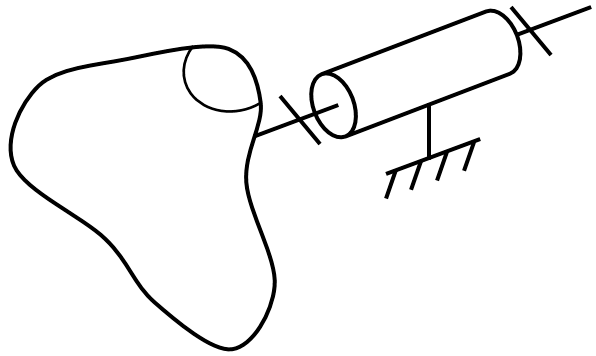
\includegraphics[width=4.5cm]{images/solide_rotation_axe_fixe.png}};
	\draw(0.77,0.9) node {\solide{S}};
	\node (A) at (0.7,-1.2) {$+$};
	\draw (A) node[above] {$M$};
	\begin{scope}[rotate=20]
		\draw[->,>=latex] (0,0)node[above] {$O$} -- (-3,0) node[above] {\vz{}};
		\draw[->,>=latex, thick] (-1.8,-0.5) arc (-90:120:0.5) node[below=1.5em, right]{$\theta$} ;
	\end{scope}
\end{tikzpicture}
	\captionof{figure}{\solide{S} en rotation autour de \axe{O}{\vz{}}}	
\end{minipage} 

\vspace{1em}
Si le centre de gravité $G$ est porté par l'axe de rotation alors : 
\[\tAM{\ext}{S}[O]=\tLigne{O}{\vNul}{J\thetapp.\vz{}}\]

\newpage
\subsection{Méthodologie du calcul du moment dynamique}

Lorsqu'on ne se trouve pas dans un de ces deux cas particuliers, le calcul se complique. Il est alors préférable de passer par la cinétique. Les calculs pouvant être très longs, il est important de les optimiser en identifiant la formule la plus adéquate à la situation considérée.

\subsubsection{Relation entre torseur cinétique et torseur dynamique}

On montre que les résultantes dynamique et cinétique sont liées par :
\[\Res{\tD{S}{\rR{g}}} = \derivV{\Res{\tC{S}{\rR{g}}}}{\rR{g}}=\derivV{(\resultanteCinetique{S}{\rR{g}})}{\rR{g}}\]

et que les moments dynamiques et cinétiques sont liés par (pour un point $A$ quelconque):
\[ \UPSTIcadreMath{\momentDynamique{A}{S}{\rR{g}} = \derivV{\momentCinetique{A}{S}{\rR{g}}}{\rR{g}}+\vVitesse{A}{}{\rR{g}}\vect m\,\vVitesse{G}{S}{\rR{g}}} \]

\begin{bclogo}[logo=\bcoutil,couleur=cyan!5,arrondi=0.1,barre=none,sousTitre=Calculer le moment dynamique]{Méthode :}
%\[ \momentDynamique{A}{S}{\rR{g}} = \derivV{\momentCinetique{A}{S}{\rR{g}}}{\rR{g}}+\vVitesse{A}{}{\rR{g}}\vect m\,\vVitesse{G}{S}{\rR{g}} \]
Cette formule permet de calculer judicieusement le moment dynamique en un point $A$ \textbf{lorsque le deuxième terme s'annule} :
\begin{itemize}
\item si $A=G$ ou $\vVitesse{A}{}{\rR{g}}//\vVitesse{G}{S}{\rR{g}}$ : $\vVitesse{A}{}{\rR{g}}\vect \vVitesse{G}{S}{\rR{g}}=\vNul$
\item si $A$ est fixe dans $\rR{g}$ : $\vVitesse{A}{}{\rR{g}}=\vNul$
\item si $G$ est fixe dans $\rR{g}$ : $\vVitesse{G}{S}{\rR{g}}=\vNul$
\end{itemize}
On a alors : $\UPSTIcadreMath{\momentDynamique{A}{S}{\rR{g}} = \derivV{\momentCinetique{A}{S}{\rR{g}}}{\rR{g}}}$

Autrement, il est plus intéressant d'utiliser la loi de changement de point des moments dynamiques (\og BABAR \fg) en passant par le point $G$.
\end{bclogo}

\subsubsection{Moment dynamique au centre de gravité $G$}

\[ \UPSTIcadreMath{\momentDynamique{G}{S}{\rR{g}} =\derivV{\momentCinetique{G}{S}{\rR{g}}}{\rR{g}}=\derivV{\left(\operateurInertie{G}{S}.\vRotation{R}{\rR{g}}\right)}{\rR{g}}}\]
\newpage
\begin{bclogo}[logo=\bcoutil,couleur=cyan!5,arrondi=0.1,barre=none,sousTitre=Calculer le moment dynamique]{Méthode :}
Si l'on n'est pas dans un des cas particuliers précédents, on utilise plutôt :
\[\momentDynamique{A}{S}{\rR{g}} =\momentDynamique{G}{S}{\rR{g}}+\vecteur{AG}\vect m\vAcceleration{G}{S}{\rR{g}}\]
\[\UPSTIcadreMath{\momentDynamique{A}{S}{\rR{g}}=\derivV{\left(\operateurInertie{G}{S}.\vRotation{R}{\rR{g}}\right)}{\rR{g}}+\vecteur{AG}\vect m\vAcceleration{G}{S}{\rR{g}}}\]
\end{bclogo}

\vspace{-1em}
\subsubsection{Moment dynamique en projection sur un axe porté par $\vz{}$}

Il est généralement inutile d'exprimer le moment dynamique dans la base globale. En effet, on applique souvent le TMD sur un axe bien choisi.

\begin{bclogo}[logo=\bcoutil,couleur=cyan!5,arrondi=0.1,barre=none,sousTitre=Calculer le moment dynamique]{Méthode :}
Si seule la composante suivant \vz{} est utile au calcul alors :
\[ \UPSTIcadreMath{\derivVl{\momentCinetique{A}{S}{\rR{g}}}{\rR{g}}\cdot \vz{}=\dfrac{d}{dt}(\momentCinetique{A}{S}{\rR{g}}\cdot \vz{})-\momentCinetique{A}{S}{\rR{g}}\cdot\derivVl{\vz{}}{\rR{g}}} \]
Dans le calcul du moment dynamique :
\[\momentDynamique{A}{S}{\rR{g}}\cdot\vz{}=\dfrac{d}{dt}(\momentCinetique{A}{S}{\rR{g}}\cdot \vz{})-\momentCinetique{A}{S}{\rR{g}}\cdot\derivVl{\vz{}}{\rR{g}}+(\vVitesse{A}{}{\rR{g}}\vect m\,\vVitesse{G}{S}{\rR{g}})\cdot\vz{}\]
Ainsi, on projette le moment cinétique avant d'en dériver toutes les composantes, et bien souvent, $\vz{}$ est un vecteur fixe de $\rR{g}$ donc sa dérivée est nulle.
\end{bclogo}

\vspace{-1em}
\subsection{Exemple : Eolienne bipale}

On s'intéresse à une éolienne bipale telle que représentée sur la figure ci-dessous.
\begin{center}
\begin{tabular}{c c c}
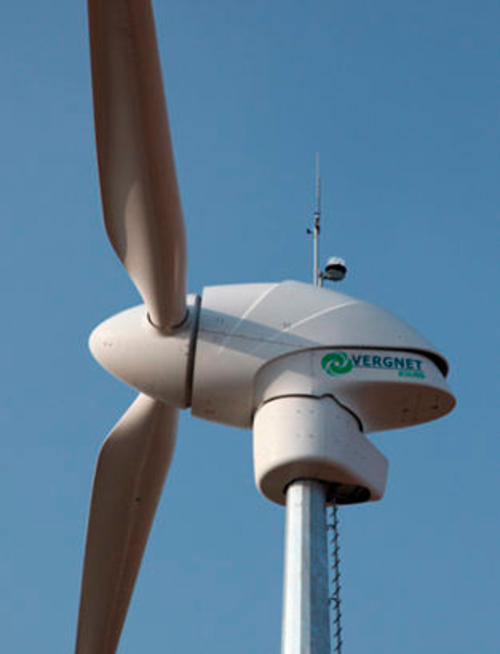
\includegraphics[width=0.3\linewidth]{images/eolienne_bipale}
& \hspace{1.5cm} &
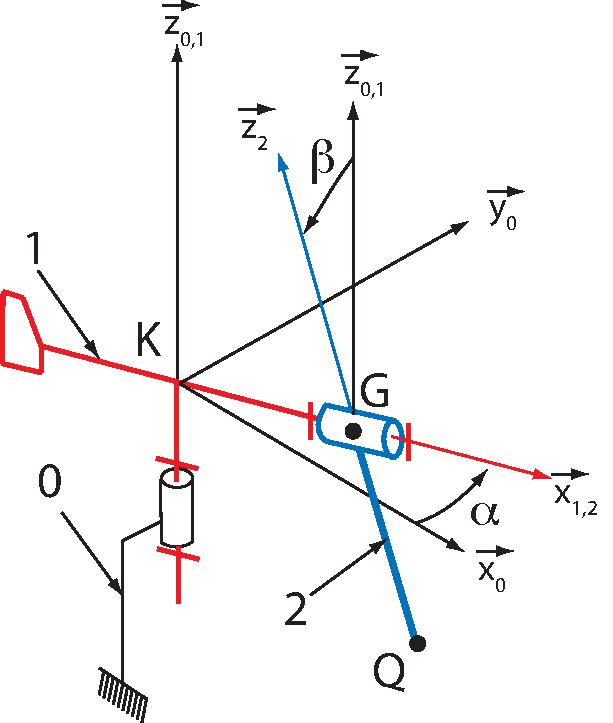
\includegraphics[width=0.33\linewidth]{images/eolienne.pdf}
\end{tabular}
\end{center}

Ce mécanisme est composé de quatre solides regroupés en  trois classes d'équivalences cinématiques :

\begin{itemize}
\item un support \textbf{0}, auquel on associe un repère $\rR0=\repere{K}{\vx0}{\vy0}{\vz0}$;
\item une girouette \textbf{1} (de centre d'inertie $K$) en liaison pivot d'axe $\couple{K}{\vz{0,1}}$ avec le support \textbf{0}. On lui associe un repère $\rR1=\repere{K}{\vx1}{\vy1}{\vz{0,1}}$ et on pose $\alpha=\couple{\vx0}{\vx1}$. On note $J$ son moment d'inertie par rapport à l'axe $\couple{K}{\vz1}$ ; %: $J=I_{\couple{K}{\vz1}}$;
\item une hélice \textbf{2}, en liaison pivot d'axe $\couple{K}{\vx{1,2}}$  avec \textbf{1}. On lui associe un repère $\rR2=\repere{K}{\vx{1,2}}{\vy2}{\vz2}$  choisi tel que $\vx2=\vx1$ et on pose $\beta=\couple{\vy1}{\vy2}$.
On note $M$ sa masse, $G$ son centre d'inertie situé sur l'axe de rotation et on pose $\vecteur{KG}=a\;\vx1$. On donne la matrice de l'opérateur d'inertie au point $G$ :
\begin{align*}
\operateurInertie{G}{2}=
\left(
\begin{array}{ccc}
A & 0 & 0 \\ 
0 & B & 0 \\ 
0 & 0 & C
\end{array}
\right)_{\base{\vx2}{\vy2}{\vz2}}
\end{align*}
\item on modélise enfin un déséquilibre possible de l'hélice en rotation par un balourd \textbf{3} assimilé à une masse ponctuelle $m$ au point $Q$. On pose $\vecteur{GQ}=-b\vz2$.
\end{itemize}

\begin{minipage}{0.5\textwidth}
%Le mécanisme a plus d'un degré de liberté.\\

On cherche à dimensionner l'actionneur permettant l'orientation de l'éolienne lorsque les effets dynamiques d'un défaut de balourd sont prépondérants.

On suppose que l'action mécanique due au moteur agissant entre $0$ et $1$ crée un couple $C_m$ selon la direction $\vz0$. 

Pour relier $C_m$ aux paramètres dynamiques du problème, on peut appliquer le théorème du moment dynamique s'appliquant sur l'éolienne $E=\left\{1+2+3\right\}$ en projection sur l'axe $\axe{K}{\vz0}$  : 
\[C_m=\left(\momentDynamique{K}{1}{0}+\momentDynamique{K}{2}{0}+\momentDynamique{K}{3}{0}\right)\cdot \vz0\]
\end{minipage}\hfill
\begin{minipage}{0.45\textwidth}
\begin{center}
\begin{tikzpicture}[scale=0.9, every node/.style={scale=0.9}]
	\node[draw, circle,fill=white](A)at(0,0){0};
	\gbati{A}
	\node[draw, circle](B)at(0,3){1};
	\node[draw, circle](C)at(3,3){2+3};
	\draw(A)to[bend left]node[pos=.6,left,align=center]{Pivot\\d'axe \axe{K}{\vz{0,1}}}(B);
	\draw[thick,<->,>=latex,double,UPSTIcustomColor1](A)to[bend right]node[midway,right]{Moteur \Cm}(B);
	\draw(B)to[bend left]node[midway,above,align=center]{Pivot\\d'axe \axe{K}{\vx{1,2}}}(C);
\end{tikzpicture}
\end{center}
\end{minipage}

\vspace{1em}
\begin{bclogo}[logo=\bcbook,couleur=DarkOrange!5,arrondi=0.1,sousTitre=Calcul de $\momentDynamique{K}{1}{0}\cdot\vz0$]{Exemple :}
\UPSTIprofEleve[1]{\np{1} est en rotation atour de l'axe fixe \axe{K}{\vz{0}}, donc $\momentDynamique{K}{1}{0}\cdot\vz0=J\alphapp$.}
{\vspace{11em}}
\end{bclogo}

\newpage
\begin{bclogo}[logo=\bcbook,couleur=DarkOrange!5,arrondi=0.1,sousTitre=Analyse de la stratégie de calcul de $\momentDynamique{K}{2}{0}\cdot\vz0$]{Exemple :}
\UPSTIprofEleve[1]{\np{2} est en rotation atour de l'axe \axe{K}{\vx{1,2}}, qui n'est pas fixe.

\noindent \underline{Solution 1 :} $K$ est un point fixe de \rR0 donc on peut utiliser la formule :
\[\momentDynamique{K}{2}{0} = \derivV{\momentCinetique{K}{2}{0}}{0}+\underbrace{\vVitesse{K}{}{0}}_{\vNul}\vect M\,\vVitesse{G}{2}{0}= \derivV{\momentCinetique{K}{2}{0}}{0}\]

\noindent Comme on cherche uniquement la projection du moment dynamique sur \vz0 :
\[\momentDynamique{K}{2}{0}\cdot\vz0 = \derivV{\momentCinetique{K}{2}{0}}{0}\cdot\vz0=\dfrac{d}{dt}(\momentCinetique{K}{2}{0}\cdot \vz0)-\momentCinetique{K}{2}{0}\cdot\underbrace{\derivVl{\vz0}{0}}_{\vNul}=\dfrac{d}{dt}(\momentCinetique{K}{2}{0}\cdot \vz0)\]
\vspace{-1em}

\noindent Cependant, l'opérateur d'inertie de \np{2} est donné en $G$ et non en $K$, le calcul de $\momentCinetique{K}{2}{0}$ n'est pas direct. On peut :
\begin{itemize}
\item soit utiliser le théorème de Huygens pour obtenir l'opérateur d'inertie en $K$ puis utiliser $\momentCinetique{K}{2}{0}=\operateurInertie{K}{2}.\vRotation{2}{0}+M\,\vecteur{KG}\vect\vVitesse{K}{2}{0}=\operateurInertie{K}{2}.\vRotation{2}{0}$ car $\vVitesse{K}{2}{0}=\vNul$ ;
\item soit utiliser la formule de changement de point du moment cinétique :\\ $\momentCinetique{K}{2}{0}=\momentCinetique{G}{2}{0}+\vecteur{KG}\vect M\vVitesse{G}{2}{0}=\operateurInertie{G}{2}.\vRotation{2}{0}+\vecteur{KG}\vect m\vVitesse{G}{2}{0}$.
\end{itemize}
Ces deux options présentent la même difficulté de calcul.

\noindent \underline{Solution 2 :} on utilise la formule de changement de point du moment dynamique
\[\momentDynamique{K}{2}{0}=\momentDynamique{G}{2}{0}+\vecteur{KG}\vect M\vAcceleration{G}{2}{0}=\derivV{\left(\operateurInertie{G}{2}.\vRotation{2}{0}\right)}{0}+\vecteur{KG}\vect M\vAcceleration{G}{2}{0}\]
puis on projette le résultat sur \vz0, ce qui reviendra au même que d'utiliser la formule de changement de point du moment cinétique, et sera légèrement plus long.

\noindent\textbf{On choisit la solution 1 avec changement de point du moment cinétique :}
\[\momentDynamique{K}{2}{0}\cdot\vz0 =\dfrac{d}{dt}(\momentCinetique{K}{2}{0}\cdot \vz0)\quad\textrm{ avec }\quad\momentCinetique{K}{2}{0}=\operateurInertie{G}{2}.\vRotation{2}{0}+\vecteur{KG}\vect M\vVitesse{G}{2}{0}\]
}
{\vspace{58em}}
\end{bclogo}

\newpage
\begin{bclogo}[logo=\bcbook,couleur=DarkOrange!5,arrondi=0.1,sousTitre=Calcul de $\momentDynamique{K}{2}{0}\cdot\vz0$]{Exemple :}
\UPSTIprofEleve[1]{
\begin{itemize}
\item Calcul de $\left(\operateurInertie{G}{2}.\vRotation{2}{0}\right)\cdot\vz0$
\end{itemize}
\noindent$\operateurInertie{G}{2}$ est donné dans la base 2 et $\vRotation{2}{0}=\vRotation{2}{1}+\vRotation{1}{0}=\betap\vx2+\alphap\vz1$.

\setCouleursParametrage{red}{red}
\parametrageAngulaire{\alpha}{\vx0}{\vy0}{\vz0}{\vx1}{\vy1}[\vz1]
\parametrageAngulaire{\beta}{\vy1}{\vz1}{\vx{1}}{\vy2}{\vz2}[\vx2]

\noindent Pour pouvoir faire le produit, on exprime $\vRotation{2}{0}$ dans la base 2 :
\[\vRotation{2}{0}=\betap\vx2+\alphap(\sin\beta\vy2+\cos\beta\vz2)\]
D'où : $\operateurInertie{G}{2}.\vRotation{2}{0}=\matriceInertie[\bB{2}][A][B][C]\vColonne{\betap \\ \alphap\sin\beta \\ \alphap\cos\beta}[\bB{2}]=\vColonne{A\betap \\ B\alphap\sin\beta \\ C\alphap\cos\beta}[\bB{2}]$\\
et $\left(\operateurInertie{G}{2}.\vRotation{2}{0}\right)\cdot\vz{0,1}=\vColonne{A\betap \\ B\alphap\sin\beta \\ C\alphap\cos\beta}[\bB{2}]\cdot\vColonne{0 \\ \sin\beta \\ \cos\beta}[\bB{2}]=\alphap(B\sin^2\beta+C\cos^2\beta)$

\begin{itemize}
\item Calcul de $\left(\vecteur{KG}\vect M\vVitesse{G}{2}{0}\right)\cdot\vz0$
\end{itemize}
$\vVitesse{G}{2}{0}=\derivV{\vecteur{KG}}{0}=a\derivV{\vx1}{0}=a\alphap\vy1$

\noindent $\vecteur{KG}\vect M\vVitesse{G}{2}{0}=a\vx1\vect M\,a\alphap\vy1=Ma^2\alphap\vz0$

\noindent d'où $\left(\vecteur{KG}\vect M\vVitesse{G}{2}{0}\right)\cdot\vz0=Ma^2\alphap$

\begin{itemize}
\item Calcul de $\momentDynamique{K}{2}{0}\cdot\vz0 =\dfrac{d}{dt}(\momentCinetique{K}{2}{0}\cdot \vz0)$
\end{itemize}
\[\dfrac{d}{dt}(\momentCinetique{K}{2}{0}\cdot \vz0)=\dfrac{d}{dt}\left(\alphap(B\sin^2\beta+C\cos^2\beta)+Ma^2\alphap\right)\]
\[\momentDynamique{K}{2}{0}\cdot\vz0=\alphapp(B\sin^2\beta+C\cos^2\beta+Ma^2)+\alphap(2B\betap\cos\beta\sin\beta-2C\betap\sin\beta\cos\beta)\]
\[\UPSTIcadreMathCor{\momentDynamique{K}{2}{0}\cdot\vz0=\alphapp(B\sin^2\beta+C\cos^2\beta+Ma^2)+\alphap\betap\sin(2\beta)(B-C)}\]
}
{\vspace{58em}}
\end{bclogo}

\newpage
\begin{bclogo}[logo=\bcbook,couleur=DarkOrange!5,arrondi=0.1,sousTitre=Analyse de la stratégie de calcul de $\momentDynamique{K}{3}{0}\cdot\vz0$]{Exemple :}
\UPSTIprofEleve[1]{\np{3} est en rotation atour de l'axe \axe{K}{\vx{1,2}}, qui n'est pas fixe.

\noindent \underline{Solution 1 :} $K$ est un point fixe de \rR0 donc on peut utiliser la formule :
\[\momentDynamique{K}{3}{0} = \derivV{\momentCinetique{K}{3}{0}}{0}+\underbrace{\vVitesse{K}{}{0}}_{\vNul}\vect m\,\vVitesse{Q}{3}{0}= \derivV{\momentCinetique{K}{3}{0}}{0}\]

\noindent Comme on cherche uniquement la projection du moment dynamique sur \vz0 :
\[\momentDynamique{K}{3}{0}\cdot\vz0 = \derivV{\momentCinetique{K}{3}{0}}{0}\cdot\vz0=\dfrac{d}{dt}(\momentCinetique{K}{3}{0}\cdot \vz0)-\momentCinetique{K}{3}{0}\cdot\underbrace{\derivVl{\vz0}{0}}_{\vNul}=\dfrac{d}{dt}(\momentCinetique{K}{3}{0}\cdot \vz0)\]
\vspace{-1em}

\noindent Le solide \np{3} est une masse ponctuelle en $Q$, donc $\operateurInertie{Q}{3}=\tenseur{0}$, $\momentCinetique{Q}{3}{0}=\vNul$ et $\momentDynamique{Q}{3}{0}=\vNul$.
Pour calculer $\momentCinetique{K}{3}{0}$, on peut :
\begin{itemize}
\item soit utiliser le théorème de Huygens pour obtenir l'opérateur d'inertie en $K$ (non nul !) puis utiliser $\momentCinetique{K}{3}{0}=\operateurInertie{K}{3}.\vRotation{3}{0}+m\,\vecteur{KQ}\vect\underbrace{\vVitesse{K}{3}{0}}_{\vNul}=\operateurInertie{K}{3}.\vRotation{3}{0}$\\
car $K$ est sur l'axe de rotation de $3/0$ ;
\item soit utiliser la formule de changement de point du moment cinétique :\\ $\momentCinetique{K}{3}{0}=\underbrace{\momentCinetique{Q}{3}{0}}_{\vNul}+\vecteur{KQ}\vect m\vVitesse{Q}{3}{0}=\vecteur{KQ}\vect m\vVitesse{Q}{3}{0}$.
\end{itemize}
La première option semble plus rapide.

\noindent \underline{Solution 2 :} on utilise la formule de changement de point du moment dynamique
\[\momentDynamique{K}{3}{0}=\underbrace{\momentDynamique{Q}{3}{0}}_{\vNul}+\vecteur{KQ}\vect m\vAcceleration{Q}{3}{0}=\vecteur{KQ}\vect m\vAcceleration{Q}{3}{0}\]
puis on projette le résultat sur \vz0, ce qui reviendra au même que d'utiliser la formule de changement de point du moment cinétique, et sera légèrement plus long.

\noindent\textbf{On choisit la solution 1 avec theorème de Huygens :}
\[\momentDynamique{K}{2}{0}\cdot\vz0 =\dfrac{d}{dt}(\momentCinetique{K}{3}{0}\cdot \vz0)\quad\textrm{ avec }\quad\momentCinetique{K}{3}{0}=\operateurInertie{K}{3}.\vRotation{3}{0}\]
}
{\vspace{58em}}
\end{bclogo}

\newpage
\begin{bclogo}[logo=\bcbook,couleur=DarkOrange!5,arrondi=0.1,sousTitre=Calcul de $\momentDynamique{K}{3}{0}\cdot\vz0$]{Exemple :}
\UPSTIprofEleve[1]{
\begin{itemize}
\item Calcul de $\operateurInertie{K}{3}$
\end{itemize}
D'après le théorème de Huygens, avec $\vecteur{KQ}=\vecteur{KG}+\vecteur{GQ}=a\vx2-b\vz2$ :
\[\operateurInertie{K}{3}=\underbrace{\operateurInertie{Q}{3}}_{\tenseur{0}}+m\matriceInertie[\bB2][b^2][a^2+b^2][a^2][0][ab]\]

\begin{itemize}
\item Calcul de $\left(\operateurInertie{K}{3}.\vRotation{3}{0}\right)\cdot\vz0$
\end{itemize}
\[\operateurInertie{K}{3}.\vRotation{3}{0}=m\matriceInertie[\bB2][b^2][a^2+b^2][a^2][0][ab]\vColonne{\betap \\ \alphap\sin\beta \\ \alphap\cos\beta}[\bB{2}]=m\vColonne{b^2\betap+ab\alphap\cos\beta \\ (a^2+b^2)\alphap\sin\beta \\ ab\betap+a^2\alphap\cos\beta}[\bB{2}]\]
car $\vRotation{3}{0}=\vRotation{2}{0}$. D'où :
\[\left(\operateurInertie{K}{3}.\vRotation{3}{0}\right)\cdot\vz0=m\vColonne{b^2\betap+ab\alphap\cos\beta \\ (a^2+b^2)\alphap\sin\beta \\ ab\betap+a^2\alphap\cos\beta}[\bB{2}]\cdot\vColonne{0 \\ \sin\beta \\ \cos\beta}[\bB{2}]\]
\[\left(\operateurInertie{K}{3}.\vRotation{3}{0}\right)\cdot\vz0=m\left[(a^2+b^2)\alphap\sin^2\beta+a^2\alphap\cos^2\beta+ab\betap\cos\beta\right]\]
\[\qquad=m\left[\alphap(a^2+b^2\sin^2\beta)+ab\betap\cos\beta\right]\]

\begin{itemize}
\item Calcul de $\momentDynamique{K}{3}{0}\cdot\vz0 =\dfrac{d}{dt}(\momentCinetique{K}{3}{0}\cdot \vz0)$
\end{itemize}
\[\momentDynamique{K}{3}{0}\cdot\vz0 =m\dfrac{d}{dt}(\alphap(a^2+b^2\sin^2\beta)+ab\betap\cos\beta)\]
\[=m\left[\alphapp(a^2+b^2\sin^2\beta)+\alphap2b^2\betap\cos\beta\sin\beta+ab\betapp\cos\beta-ab\betap^2\sin\beta\right]\]
\[\UPSTIcadreMathCor{\momentDynamique{K}{3}{0}\cdot\vz0 =m\left[\alphapp(a^2+b^2\sin^2\beta)+\alphap\betap b^2\sin(2\beta)+ab\betapp\cos\beta-ab\betap^2\sin\beta\right]}\]
}
{\vspace{58em}}
\end{bclogo}

%%%%%%%%%%%%%%%%%%%
%Annexes
%%%%%%%%%%%%%%%%%%%
\newpage
\section{Annexes}

\subsection{Preuve que les moments dynamiques forment un champ de torseur}

On vérifie que les moments forment un champ de torseur.

\noindent On a : $\vecteur{AM}=\vecteur{AB}+\vecteur{BM}$ avec $A$ et $B$ deux points fixes de \solide{S}, et $M$ décrivant le solide \solide{S}.

\noindent On peut alors décomposer le terme $\displaystyle{\int_S}\vecteur{AM}\vect \vAcceleration{M}{S}{\rR{g}} dm$:
\begin{flalign*}
	& \int_S\vecteur{AM}\vect \vAcceleration{M}{S}{\rR{g}} dm=\int_S\vecteur{AB}\vect \vAcceleration{M}{S}{\rR{g}} dm+\int_S\vecteur{BM}\vect \vAcceleration{M}{S}{\rR{g}} dm \quad\textrm{(relation de Chasles)}&\\
	& \int_S\vecteur{AM}\vect \vAcceleration{M}{S}{\rR{g}} dm=\vecteur{AB}\vect\int_S\vAcceleration{M}{S}{\rR{g}} dm+\int_S\vecteur{BM}\vect \vAcceleration{M}{S}{\rR{g}} dm \quad\textrm{(car $AB=\cste$)} \\
	& \underbrace{\int_S\vecteur{AM}\vect \vAcceleration{M}{S}{\rR{g}} dm}_\text{Moment en $A$}=\underbrace{\int_S\vecteur{BM}\vect \vAcceleration{M}{S}{\rR{g}} dm}_\text{Moment en $B$} +\vecteur{AB}\vect \underbrace{m\,\vAcceleration{G}{S}{\rR{g}}}_\text{Résultante}
\end{flalign*}

\subsection{Moment dynamique pour un solide en translation}

\subsubsection{Moment dynamique en $G$}
\vspace{-1em}
\begin{flalign*}
	& \momentDynamique{G}{S}{\rR{g}}=\momentDynamiqueDef{G}{S}{\rR{g}}=\int_S \vecteur{GM}\vect\vAcceleration{G}{S}{\rR{g}} dm \quad\textrm{(Translation)} &\\
	& \momentDynamique{G}{S}{\rR{g}}=\int_S \vecteur{GO}\vect\vAcceleration{G}{S}{\rR{g}}dm+\int_S \vecteur{OM}\vect\vAcceleration{G}{S}{\rR{g}}dm\quad \textrm{(relation de Chasles)} \\
	& \momentDynamique{G}{S}{\rR{g}}=\vecteur{GO}\vect\vAcceleration{G}{S}{\rR{g}} \int_S dm+\left(\int_S \vOM dm\right)\vect \vAcceleration{G}{S}{\rR{g}} \quad\textrm{($O$ et $G$ fixes / \solide{S})} \\
	& \momentDynamique{G}{S}{\rR{g}}=\vecteur{GO}\vect m\,\vAcceleration{G}{S}{\rR{g}}+m\,\vOG\vect\vAcceleration{G}{S}{\rR{g}} \quad\textrm{(Définition du centre de gravité)}\\
	& \momentDynamique{G}{S}{\rR{g}}=\vNul
\end{flalign*}

\subsubsection{Moment dynamique en un point quelconque $A$}
\vspace{-1em}
\begin{flalign*}
	& \momentDynamique{A}{S}{\rR{g}}=\momentDynamiqueDef{A}{S}{\rR{g}}=\int_S \vecteur{AM}\vect\vAcceleration{G}{S}{\rR{g}}dm \quad\textrm{(Translation)} &\\
	& \momentDynamique{A}{S}{\rR{g}}=\int_S \vecteur{AG}\vect\vAcceleration{G}{S}{\rR{g}}dm+\int_S \vecteur{GM}\vect\vAcceleration{G}{S}{\rR{g}}dm\quad\textrm{(relation de Chasles)} \\
	& \momentDynamique{A}{S}{\rR{g}}=\vecteur{AG}\vect\vAcceleration{G}{S}{\rR{g}} \int_S dm+\momentDynamique{G}{S}{\rR{g}} \quad\textrm{($O$ et $G$ fixes / \solide{S})} \\
	& \momentDynamique{A}{S}{\rR{g}}=m\,\vecteur{AG}\vect\vAcceleration{G}{S}{\rR{g}}
\end{flalign*}

\subsection{Moment dynamique pour un solide en rotation autour d'un axe fixe \axe{O}{\vz{}}}

Avec $r$ la distance orthogonale de $M$ à l'axe $\axe{O}{\vz{}}$, pour une rotation d'angle $\theta$, on a :
\begin{flalign*}
	& \momentDynamique{O}{S}{\rR{g}}=\momentDynamiqueDef{O}{S}{\rR{g}} &\\
	& \momentDynamique{O}{S}{\rR{g}}=\int_S r.\vu{}\vect\left(-r\thetap^2.\vu{}+r\thetapp.\vecteur{v}\right) dm=\int_S r^2\thetapp dm.\vz{}=\thetapp\int_S r^2dm.\vz{}=J.\thetapp\vz{} \\
	& \text{Avec le moment d'inertie : } J=\int_S r^2dm
\end{flalign*}

\vspace{-1em}
\subsection{Preuve du lien entre torseur cinétique et torseur dynamique}

\subsubsection{Résultantes}

$\Res{\tC{S}{\rR{g}}} = \resultanteCinetiqueDef{S}{\rR{g}} = \resultanteCinetique{S}{\rR{g}}$ et 
$\Res{\tD{S}{\rR{g}}} = \resultanteDynamiqueDef{S}{\rR{g}} = \resultanteDynamique{S}{\rR{g}}$

\noindent Or, $\vAcceleration{G}{S}{\rR{g}}=\derivV{\vVitesse{G}{S}{\rR{g}}}{\rR{g}}$, d'où $\Res{\tD{S}{\rR{g}}} = \derivV{\Res{\tC{S}{\rR{g}}}}{\rR{g}}$

\vspace{-1.5em}
\subsubsection{Moments}

$\momentCinetique{A}{S}{\rR{g}}=\momentCinetiqueDef{A}{S}{\rR{g}}$ et $\momentDynamique{A}{S}{\rR{g}}=\momentDynamiqueDef{A}{S}{\rR{g}}$

\noindent Dérivons le moment cinétique :
\begin{flalign*}
	& \derivV{\momentCinetique{A}{S}{\rR{g}}}{\rR{g}}=\int_S \derivV{\vecteur{AM}\vect\vVitesse{M}{S}{\rR{g}}}{\rR{g}}dm \\
	& \derivV{\momentCinetique{A}{S}{\rR{g}}}{\rR{g}}=\int_S \derivV{\vecteur{AM}}{\rR{g}}\vect\vVitesse{M}{S}{\rR{g}}dm+\int_S\vecteur{AM}\vect\derivV{\vVitesse{M}{S}{\rR{g}}}{\rR{g}}dm
\end{flalign*}
\noindent Or, $\derivV{\vecteur{AM}}{\rR{g}}=\derivV{\vecteur{AO}}{\rR{g}}+\derivV{\vecteur{OM}}{\rR{g}}=-\vVitesse{A}{}{\rR{g}}+\vVitesse{M}{}{\rR{g}}$, d'où :
\begin{flalign*}
	& \derivV{\momentCinetique{A}{S}{\rR{g}}}{\rR{g}}=\int_S \left(-\vVitesse{A}{}{\rR{g}}+\vVitesse{M}{}{\rR{g}}\right)\vect\vVitesse{M}{}{\rR{g}}dm+\int_S\vecteur{AM}\vect\vAcceleration{M}{}{\rR{g}}dm\\
	& \derivV{\momentCinetique{A}{S}{\rR{g}}}{\rR{g}}=\int_S \left(-\vVitesse{A}{}{\rR{g}}\vect\vVitesse{M}{}{\rR{g}}+\vVitesse{M}{}{\rR{g}}\vect\vVitesse{M}{}{\rR{g}}\right)dm+\momentDynamique{A}{S}{\rR{g}}\\
	& \derivV{\momentCinetique{A}{S}{\rR{g}}}{\rR{g}}=-\vVitesse{A}{}{\rR{g}}\vect\int_S\vVitesse{M}{}{\rR{g}}dm+\momentDynamique{A}{S}{\rR{g}}
\end{flalign*}
Ainsi, $\momentDynamique{A}{S}{\rR{g}} = \derivV{\momentCinetique{A}{S}{\rR{g}}}{\rR{g}}+\vVitesse{A}{}{\rR{g}}\vect m\,\vVitesse{G}{S}{\rR{g}}$.


\end{document}












